\documentclass[9pt]{beamer}

%\usetheme{Marburg}
\usetheme{Goettingen}

% package list
\usepackage{graphicx}
\usepackage{wrapfig}

% prensentation info
\title{{A framework of salient object detection for images and videos}}
\author{Jimmy Lin}
\institute{supervised by Dr. Stephen Gould\\ College of Engineering and Computer Science \\Australian National University}
\date{\today}

% new command definition
\DeclareMathOperator*{\argmin}{arg\,min}
\DeclareMathOperator*{\argmax}{arg\,max}


%%% beginning of document
\begin{document}
\begin{large}
\frame{\titlepage }
\end{large}

% Motivation
\section{1 Motivation}
\begin{large}
\frame {
    \frametitle{Problem Motivation}
    \begin{itemize}
        \item What is salient object? \vspace{0.2cm}\\
            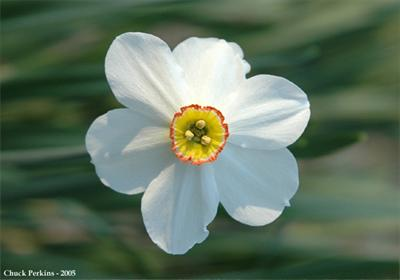
\includegraphics[width=1.6in,height=1.15in]{Picture/PM1.jpg} \hspace{0.1cm}
            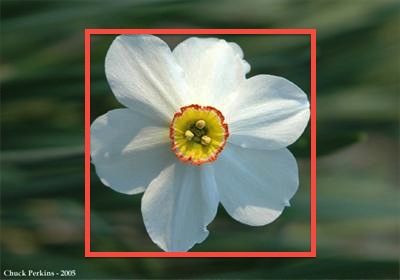
\includegraphics[width=1.6in,height=1.15in]{Picture/PM.jpg} \\
            \begin{center} \figcaption{\footnotesize Fig. images from MSRA datasets B} \end{center}
            \begin{itemize} % only for image
                \item high contrast in object's boundary
                \item intensive color spatial distribution
                \item spatial / temporal continuity
            \end{itemize}

        \item Why to detect salient objects? %A technique simulating human attention
            \begin{itemize}
                \item Adaptive image display on small devices
                \item Automatic image cropping
                \item Image/video compression
                \item ...
            \end{itemize}

    \end{itemize}
}
\end{large}

% related work
\section{2 Related Works}
\frame{
    \frametitle{Related Works}
    \begin{itemize}
        \item Salient-based Model (SM,1998) \\
        \begin{thebibliography}{9}
        \footnotesize
        \bibitem{ConcreteMath} Itti, Laurent, Christof Koch, and Ernst Niebur. "A model of saliency-based visual attention for rapid scene analysis."\textit{ Pattern Analysis and Machine Intelligence, IEEE Transactions on 20.11 (1998): 1254-1259.}
    \end{thebibliography}

    \item Fuzzy Growing Method (FG,2003) \\
        \begin{thebibliography}{9}
            \footnotesize
            \bibitem{ConcreteMath} Ma, Yu-Fei, and Hong-Jiang Zhang. "Contrast-based image attention analysis by using fuzzy growing."\textit{ Proceedings of the eleventh ACM international conference on Multimedia. ACM, 2003.} 
            \end{thebibliography}
    \item CRF-based Model (CRFM,2007)
        \begin{thebibliography}{9}
            \footnotesize 
            \bibitem{ConcreteMath} Liu, Tie, et al. "Learning to detect a salient object."\textit{ Computer Vision and Pattern Recognition, 2007. CVPR'07. IEEE Conference on. IEEE, 2007. }
            \bibitem Liu, Tie, et al. "Learning to detect a salient object."\textit{ Pattern Analysis and Machine Intelligence, IEEE Transactions on 33.2 (2011): 353-367.}
        \end{thebibliography}
    \end{itemize}
    \begin{center}
    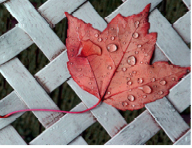
\includegraphics[width=1.1in,height=0.8in]{Picture/feature_maps/original_Image.png} \hspace{0.1cm}
    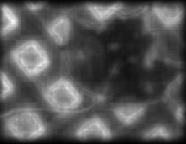
\includegraphics[width=1.1in,height=0.8in]{Picture/feature_maps/Itti_feature_map.png} \hspace{0.1cm}
    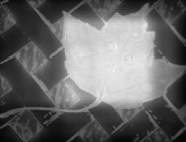
\includegraphics[width=1.1in,height=0.8in]{Picture/feature_maps/ours_feature_map.png} \hspace{0.1cm} \\
    \figcaption{\footnotesize (a) input image (b) feature map of SM (c) feature map of CRFM}
    \end{center}
}

% Formulation
\section{3 Formulation}
\frame{
    \frametitle{Problem Formulation}
    \begin{itemize}
    \item Binary Labelling Task, \\
    \qquad For each pixel $x$, $a_{x} \in \{0,1\}$ indicate whether pixel x belongs to salient object. \\

    \item For image, \\
    \qquad One single image $I$, \\
    \qquad Corresponding Binary Mask $A$, \\
    \qquad Probabilistic model $P(A|I) = \frac{1}{Z} exp(-E(A|I))$. \\

    \item For video, \\
    \qquad A sequence of image $I_{1},I_{2}...I_{N}$, \\
    \qquad Corresponding sequence of Binary Mask $A_{1},A_{2}...A_{N}$, \\
    \qquad PM $P(A_{1,...,N}|I_{1,...,N}) = \frac{1}{Z} exp(-E(A_{1,...,N}|I_{1,...,N})) $.  \vspace{-0.1cm} \\
    $$ E(A_{1,...,N}|I_{1,...,N}) 
        = \sum_{t=1}^{N} E(A_{t}|I_{1,...,N}) 
        = \sum_{t=1}^{N} E(A_{t}|I_{t-1},I_{t}) $$
    
    \item Formulating Energy Function \\
    \item Learning and Inference for CRF model \\
    \item Evaluating the result of model
\end{itemize}
}

% Formulation in a single image
\subsection{a. of a single image}
\frame{
    \frametitle{Formulation in a single image}
    Energy function is formualted as
    $$ E(A|I) = \sum_{x} \sum_{k=1}^{K} \lambda_{k} F_{k}(a_{x},I)  
        + \sum_{x,x'} S(a_{x},a_{x'},I)  $$ \vspace{-0.4cm} \\
    \begin{small}
        \qquad $\lambda_{k}$: weight of $k$th feature, $x,x'$: two adjacent pixels. \\
    \end{small}
    \textbf{Static salient feature.} $F_{k} (a_{x},I)$ is formulated from a normalized feature map $f_{k} (x,I) \in [0,1]$ for every pixel, written as:
    $$ F_{k} (a_{x},I) = 
        \begin{cases}
        f_{k} (x,I),   & { a_{x} = 0 } \\
        1-f_{k} (x,I), & { a_{x} = 1 } 
        \end{cases}
    \right.
    $$  

    \textbf{Pairwise feature.} $S(a_{x},a_{x'},I)$ exploits the spatial relationship between two adjacent pixels and can be viewed as a penalty to adjacent pixels that are assigned with different labels. 
    $$ S(a_{x},a_{x'},I) = |a_{x} - a_{x'}| \cdot exp(-\beta d_{x,x'}) $$
    \qquad where $ d_{x,x'} = ||I_{x}-I_{x'}||_{2}$ is the L2-norm of color difference, 
     and $\beta = (2 \langle ||I_{x}-I_{x'}||^{2} \rangle)^{-1}$ is robust parameter weighting the color contrast.
     \vspace{0.05cm} \\
    \hrule
    \begin{thebibliography}{9}
        \tiny
        \bibitem{ConcreteMath} Liu, Tie, et al. "Learning to detect a salient object."\textit{ Computer Vision and Pattern Recognition, 2007. CVPR'07. IEEE Conference on. IEEE, 2007. }
    \end{thebibliography}
}
% Formulation in sequential images
\subsection{b. of sequential images}
\frame{
    \frametitle{Formulation in sequential images}
    Energy function is formulated as 
    $$ E(A_{t}|I_{t},I_{t-1}) = 
    \sum_{x} \Big(
        \sum_{k=1}^{K} \lambda_{k} F_{k} (a_{x},I_{t}) +
        \sum_{k=K+1}^{K+L} \lambda_{k} F_{k} (a_{x},M_{t}) \vspace{-0.3cm} \\
        \qquad \qquad \qquad \qquad +\lambda_{0} F(a_{x},I_{t-1},I_{t})
        \Big) + S(a_{x},a_{x'},I_{t}) ,
    $$  \\
    \textbf{Motion salient features.} Processing is similar to Static salient features, but based on motion field $M_{t}$ of the image $I_{t}$. The motion field is obtained by using the SIFT flow technique. 
        \begin{center}
    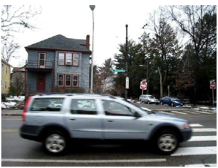
\includegraphics[width=0.8in,height=0.6in]{Picture/motionField/A.png} 
    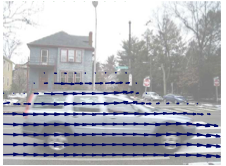
\includegraphics[width=0.8in,height=0.6in]{Picture/motionField/Am.png} \hspace{0.1cm} \\
    \figcaption{\footnotesize Fig. (a) Original Image (b) Motion Field }
    \end{center}
    \textbf{Appearance coherent feature.} This feature $f(x,I_{t-1},I_{t})$ penalizes the pixels that are identified to be in the salient object, but with a large color difference between the surrounding regions from two adjacent frames.
         \vspace{0.3cm} \\
    \hrule
    \begin{thebibliography}{9}
        \tiny
        \bibitem{ConcreteMath} Liu, Tie, et al. "Learning to detect a salient object."\textit{ Computer Vision and Pattern Recognition, 2007. CVPR'07. IEEE Conference on. IEEE, 2007. } 
        \bibitem{ConcreteMath} Liu, Ce, et al. "SIFT flow: dense correspondence across different scenes."\textit{ Computer Vision–ECCV 2008. Springer Berlin Heidelberg, 2008. 28-42.}
    \end{thebibliography}
}

\section{4 Static Salient Features}
% Local feature
\subsection{a. Multiscale Constrast}
\frame{
    \frametitle{Local Feature: Multiscale Contrast}
    Contrast is the most commonly used local feature for attention detection because it simulates the human visual receptive fields. \vspace{0.1cm} \\
    \begin{center}
    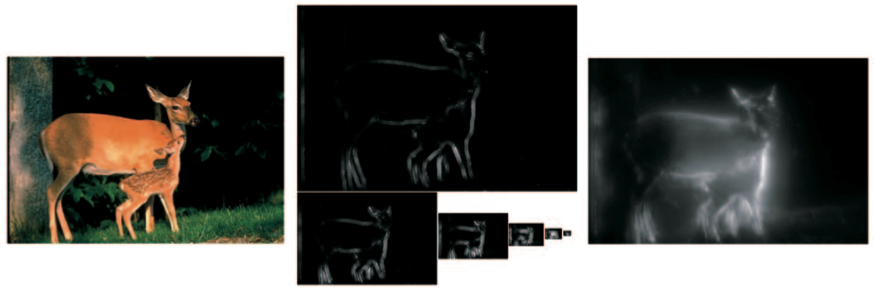
\includegraphics[width=3.5in,height=1.0in]{picture/Multiscale_Contrast.png} \\
    \figcaption{\footnotesize  (a) Input image (b) Contrast maps at multiple scales (c) feature map\\}
    \end{center}
    Multiscale contrast feature $f_{c}(x,I)$ is defined as a linear combination of contrasts in the Gaussian image pyramid:
    $$ f_{c} (x,I) = \sum_{q=1}^{Q} \sum_{x' \in N(x)} || I^{q}(x) - I^{q}(x')||^{2}$$
    \qquad where $ N(x) $ is $ 9 \times 9 $ windows, $q$ is the index for the scales in pyramid.  
    %\qquad where, $I^{l}$ is the $l$th-level image in the pyramid and the number of pyramid levels L is 6. $N(x)$ is a $9 \times 9$ window. \\
    \hrule
    \begin{thebibliography}{9}
        \tiny
        \bibitem{ConcreteMath} Liu, Tie, et al. "Learning to detect a salient object."\textit{ Computer Vision and Pattern Recognition, 2007. CVPR'07. IEEE Conference on. IEEE, 2007. }
    \end{thebibliography}
}
% Regional feature
\subsection{b. CS histogram}
\frame{
    \frametitle{Regional Feature: Center-Surround Histogram}
    Find the most distinct rectangle, $R^{*}(x)$, centered at each pixel $x$ by varying the size and aspect ratio:  
    $$ R^{*}(x) = \argmax_{R(x)}\chi^{2} (R(x),R_{S}(x)) $$
    %$$ \chi^{2} (R,R_{S}) = \frac{1}{2} \sum_{i} \frac{(R^{i} - R_{S}^{i})^{2}}{ R^{i} + R_{S}^{i}} $$ \\
    \qquad Five templates of aspect ratios $\{0.5, 0.75, 1.0, 1.5, 2.0\}$. \\
    \qquad Size range of rectangle $ R(x)$ can be set as $[0.1, 0.7] \times min(w,h) $.  \vspace{0.2cm} \\
    \begin{center}
        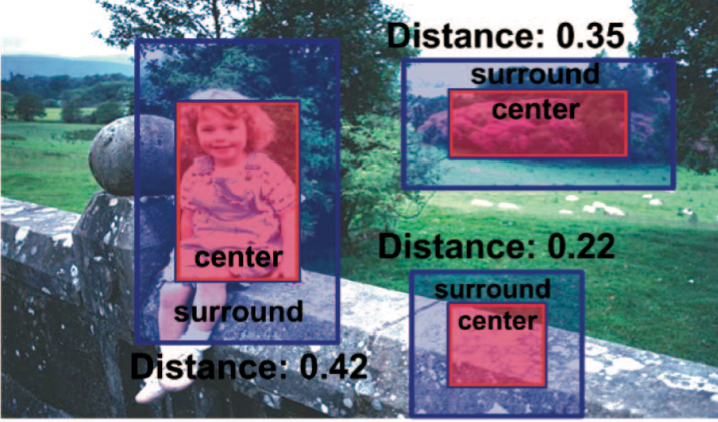
\includegraphics[width=4.0cm,height=2.5cm]{picture/Histogram.png} \hspace{0.2cm}
        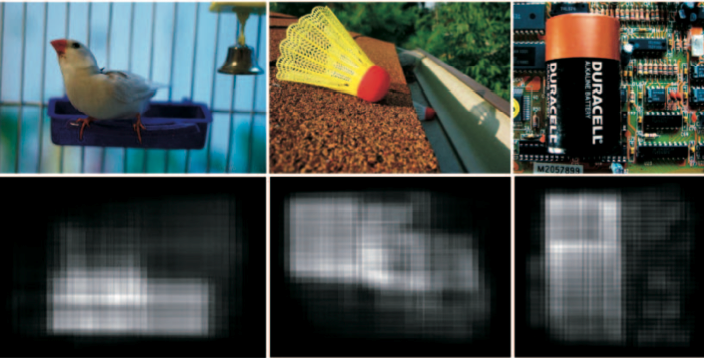
\includegraphics[width=4.0cm,height=2.5cm]{picture/Histogram_featuremaps.png} \\
        \figcaption{\footnotesize (a) Center-Surround Histogram (b)Feature Maps of Center-Surround Histogram}
    \end{center}
    % where $\chi^{2}$ distance between histograms of two rectangles is,
    The center-surround histogram feature $f_{h}(x,I)$ is defined as 
    $$ f_{h}(x,I) \propto \sum_{\{x'|x \in R^{*}(x')\} } w_{xx'} \chi^{2} (R^{*}(x'), R_{S}^{*}(x')) $$

        \hrule
    \begin{thebibliography}{9}
        \tiny
        \bibitem{ConcreteMath} Liu, Tie, et al. "Learning to detect a salient object."\textit{ Computer Vision and Pattern Recognition, 2007. CVPR'07. IEEE Conference on. IEEE, 2007. }
    \end{thebibliography}
}
% Global feature
\subsection{c. Color Spatial Distribution}
\frame{
    \frametitle{Global Feature: Color Spatial Distribution}
    We use Gaussian Mixture Models (GMMs) $\{w_{c},\mu_{c},\Sigma_{c}\}_{c=1}^{C}$ to represent all colors in the image. Each pixel is assigned to a color component with the probability
    $$ P(c|I_{x}) = \frac{w_{c} \mathcal{N}(I_{x}|\mu_{c}, \sigma_{c})}
    {\sum_{c} w_{c} \mathcal{N}(I_{x}|\mu_{c}, \sum_{c})} $$
%    Derive the horizontal variance of color component by:
%    $$ V_{h} = \frac{1}{|X|_{c}}\sum_{x}p(c|I_{x}) \cdot |x_{h}-M_{h}|^{2} $$
%    \qquad where $ M_{h}(c) = \frac{1}{|X|_{c}} \sum_{x} p(c|I_{x}) \cdot x_{h} $ 
%            and $ |X|_{c} = \sum_{x} p(c|I_{x}) $ \vspace{0.2cm} \\
%    Similarly, derive vertical variance $ V_{v} $ and form the spatial variance,
%    $$ V(c) = V_{h}(c) + V_{v}(c) $$
    \begin{center}
    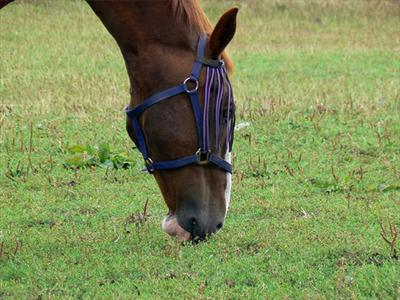
\includegraphics[width=1.0in,height=0.8in]{Picture/globalFeature/A.jpg} \hspace{0.1cm}
    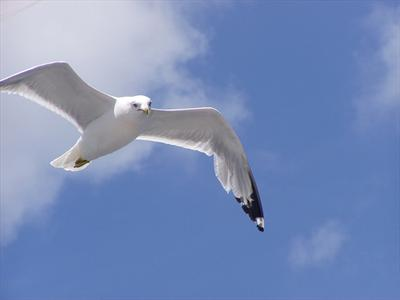
\includegraphics[width=1.0in,height=0.8in]{Picture/globalFeature/B.jpg} \hspace{0.1cm}
    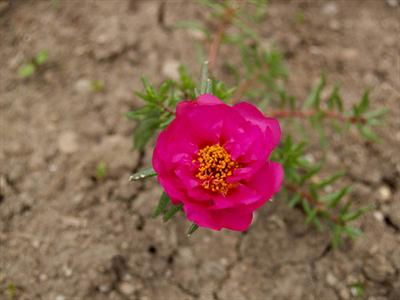
\includegraphics[width=1.0in,height=0.8in]{Picture/globalFeature/C.jpg} \hspace{0.1cm} \\
    \figcaption{\footnotesize Fig. three examples making use of global feature (a) grass (b) sky (c) soil }
    \end{center}
    Then we compute composite variance and normalize it to $[0,1]$. Finally define the color spatial-distribution feature as,
    $$ f_{s}(x,I) \propto \sum_{c} p(c|I_{x}) \cdot (1-V(c))$$

        \hrule
    \begin{thebibliography}{9}
        \tiny
        \bibitem{ConcreteMath} Liu, Tie, et al. "Learning to detect a salient object."\textit{ Computer Vision and Pattern Recognition, 2007. CVPR'07. IEEE Conference on. IEEE, 2007. }
    \end{thebibliography}
}

% Dynamic features
%\section{4 Motion Salient Features}
%\frame{
%    \frametitle{Motion Salient Features}
%    Multiscale contrast of weighted motion field.
%    $$ f_{M_{c}}(x,M) = \sum_{l=1}^{L} \sum_{x' \in N(x)} 
%            W_{x}^{l} W_{x'}^{l} 
%                || M^{l}(x) - M^{l} (x') || $$
%    \qquad where $M^{l}$ is the $l$th-level motion in the pyramid. \vspace{0.2cm} \\
%    Center-surround histogram of weighted motion field.
%    $$ f_{M_{h}} (x,M) \propto \sum_{x'| x \in R_{M}^{*}(x')} 
%            w_{xx'} W_{x'} \chi^{2} (R_{M}^{*}, R_{M_{S}}^{*}(x')) $$
%    \qquad where $R_{M}^{*}$ is the rectangle with largest center-surround histogram distance on motion vectors, and $w_{xx'}$ is the weight for the spatial distance. \vspace{0.2cm}\\
%    Spatial distribution of weighted motion field. To get the spatial distribution, these motion vectors weighted by $W_{x}$ are first clustered into several GMMs. The spatial variance $V(m)$ of each Gaussian component $m$ is computed similar to the color spatial distribution.
%    $$ f_{M_{s} (x,M)} \propto \sum_{m} W_{x} p(m|M_{x}) \cdot (1-V_{M}(m)) $$
%}

% Appearance Coherence
%\section{5 Appearance Coherence}
%\frame{
%    \frametitle{Appearance Coherence}
%    Supposition: Salient objects from two consecutive frames probably have similar appearance features. \\
%    Penalize the pixels that are identified to be in the salient object by static salient features but with a big color histogram difference. \\
%    First, compute the weighted color histogram $R_{t}(x)$ from $N^{2}$ surrounding pixel, $b$th bin of the color histogram is given by
%    $$ R_{t}(x)^{b} = \sum_{x' \in R_{t}} f(x',I) \delta (I_{x'} = b)  $$
%    Second, search the patch in the image $I_{t}$ to find the rectangle with largest distance to $R_{t}(x)$
%    $$ R_{t-1}(x') = \argmax_{x'} \chi^{2} (R_{t}(x), R_{t-1}(x'))$$
%    $$ f(x,I_{t},I_{t-1}) \propto \frac{f(x,I_{t}) + f(x^{*},I_{t})}{2} 
%        exp(-\chi^{2} (R_{t}(x),R_{t-1}(x^{*}))) $$
%    \qquad where $f(x,I_{t})$ $f(x^{*},I_{t}) $ are the static salient features from $I_{t}$ and $I_{t-1}$ 
%}

\section{5. Evaluation}
% CRF learning
\subsection{a. Learning}
% CRF inference
\subsection{b. Inference}

% Evaluation
\subsection{c. Criteria}
\frame{
    \frametitle{Evaluation Criteria}
    \begin{itemize}
        \item Region-based measurement \\
            \begin{center}
            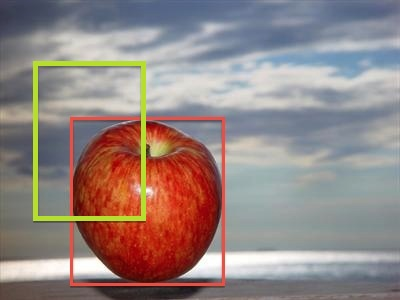
\includegraphics[width=1.0in,height=0.8in]{Picture/Creteria/A.jpg} \hspace{0.1cm}
            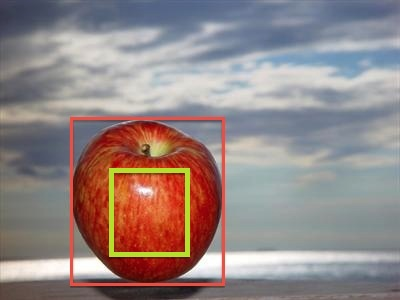
\includegraphics[width=1.0in,height=0.8in]{Picture/Creteria/B.jpg} \hspace{0.1cm}
            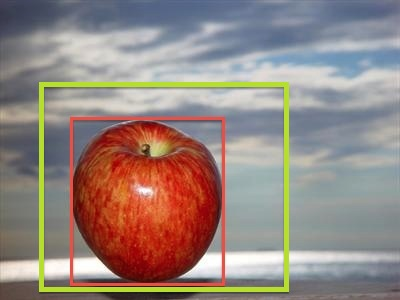
\includegraphics[width=1.0in,height=0.8in]{Picture/Creteria/C.jpg} \hspace{0.1cm} \\
            \figcaption{\footnotesize (a) arbitrary labelling (b) large prec but low recall (c) large recall but low prec}
            \end{center}
            \begin{itemize}
                \item Ratio of Precision to Recall \\
                    Precision: \% of pixels that are correctly detected in ground truth\\ 
                    Recall: \% of pixels that are correctly detected in resulted detection\\
                \item F-Measure
    $$ F_{\alpha} = \frac{(1+\alpha) \times{Precision}\times{Recall}} {\alpha \times Precision + Recall} $$
            \end{itemize}
        \item Boundary-based measurement
            \begin{itemize}
                \item Boundary Displacement Error (BDE) \\
                    Measures the average of positional difference of ground truth and resulted detection.

            \end{itemize}
    \end{itemize}

            \hrule
    \begin{thebibliography}{9}
        \tiny
        \bibitem{ConcreteMath} Liu, Tie, et al. "Learning to detect a salient object."\textit{ Computer Vision and Pattern Recognition, 2007. CVPR'07. IEEE Conference on. IEEE, 2007. }
    \end{thebibliography}
}

\section{6 Comparisons}
\subsection{a. perfect}
\frame{
    \frametitle{Result Comparisons: perfect detection}
    \centering
    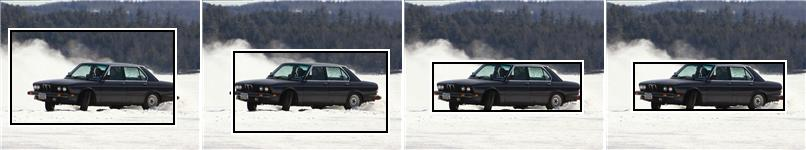
\includegraphics[width=1.9in,height=0.8in]{picture/perfectComparison/35_imCanvs_Compare.jpg} 
    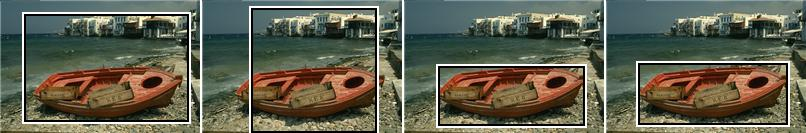
\includegraphics[width=1.9in,height=0.8in]{picture/perfectComparison/18_imCanvs_Compare.jpg} \\
    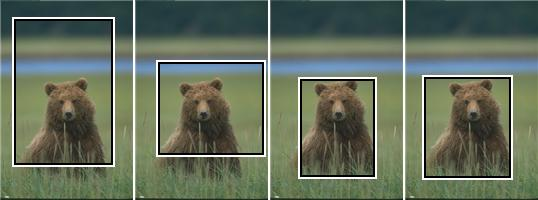
\includegraphics[width=1.9in,height=0.8in]{picture/perfectComparison/3_imCanvs_Compare.jpg} 
    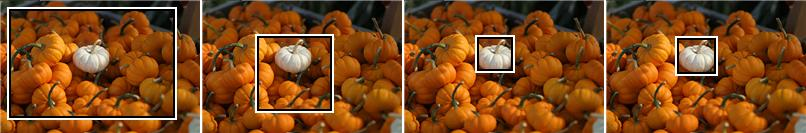
\includegraphics[width=1.9in,height=0.8in]{picture/perfectComparison/10_imCanvs_Compare.jpg} \\
    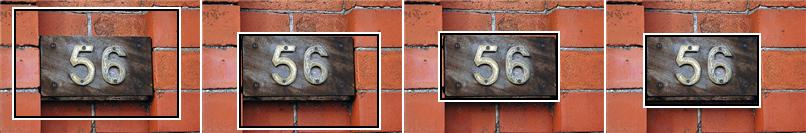
\includegraphics[width=1.9in,height=0.8in]{picture/perfectComparison/67_imCanvs_Compare.jpg}
    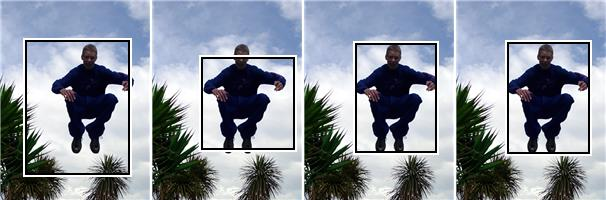
\includegraphics[width=1.9in,height=0.8in]{picture/perfectComparison/0_imCanvs_Compare.jpg} \\
    \figcaption{\footnotesize (a) FG(Ma,2003) (b) SM(Itti,1998) (c) CRFM(Liu,2007) (d) Ground truth\vspace{0.3cm} \\}
    \hrule
    \begin{thebibliography}{9}
        \tiny
        \bibitem{ConcreteMath} Liu, Tie, et al. "Learning to detect a salient object."\textit{ Computer Vision and Pattern Recognition, 2007. CVPR'07. IEEE Conference on. IEEE, 2007. }
    \end{thebibliography}
}
\subsection{b. just-so-so}
\frame{
    \frametitle{Result Comparisons: decent detection}
    \centering
    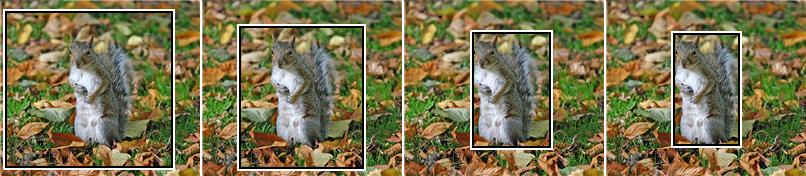
\includegraphics[width=1.9in,height=0.8in]{picture/sosoComparison/13_imCanvs_Compare.jpg} 
    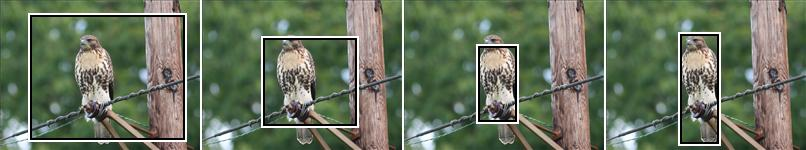
\includegraphics[width=1.9in,height=0.8in]{picture/sosoComparison/159_imCanvs_Compare.jpg} \\
    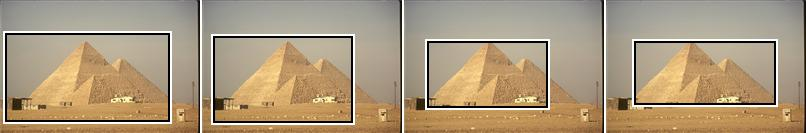
\includegraphics[width=1.9in,height=0.8in]{picture/sosoComparison/41_imCanvs_Compare.jpg} 
    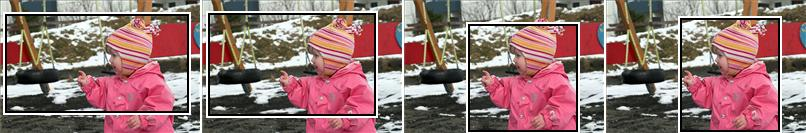
\includegraphics[width=1.9in,height=0.8in]{picture/sosoComparison/44_imCanvs_Compare.jpg} \\
    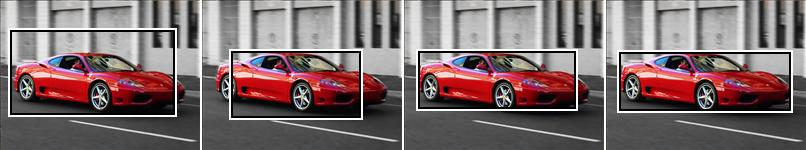
\includegraphics[width=1.9in,height=0.8in]{picture/sosoComparison/71_imCanvs_Compare.jpg}
    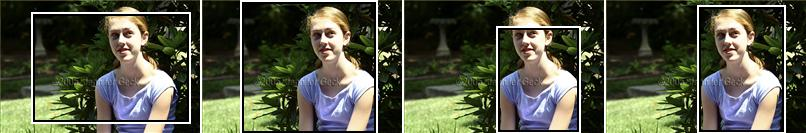
\includegraphics[width=1.9in,height=0.8in]{picture/sosoComparison/89_imCanvs_Compare.jpg} \\
    \figcaption{\footnotesize (a) FG(Ma,2003) (b) SM(Itti,1998) (c) CRFM(Liu,2007) (d) Ground truth\vspace{0.3cm}  \\}
    \hrule
    \begin{thebibliography}{9}
        \tiny
        \bibitem{ConcreteMath} Liu, Tie, et al. "Learning to detect a salient object."\textit{ Computer Vision and Pattern Recognition, 2007. CVPR'07. IEEE Conference on. IEEE, 2007. }
    \end{thebibliography}


}
\subsection{c. terrible}
\frame{
    \frametitle{Result Comparisons: terrible detection}
    \centering
    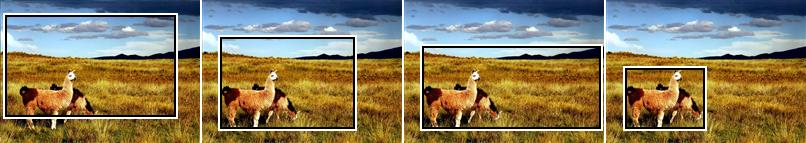
\includegraphics[width=1.9in,height=0.8in]{picture/badComparison/6_185_compare.jpg} 
    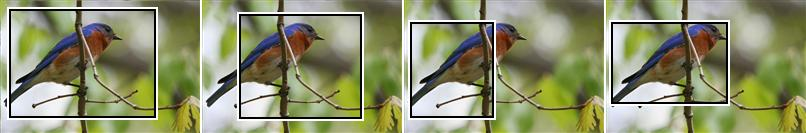
\includegraphics[width=1.9in,height=0.8in]{picture/badComparison/6_212_compare.jpg} \\
    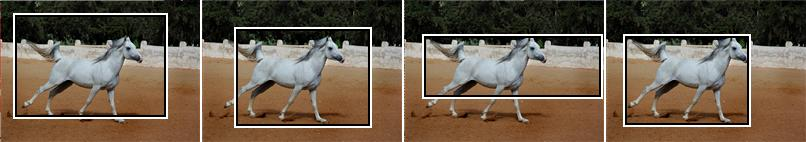
\includegraphics[width=1.9in,height=0.8in]{picture/badComparison/6_301_compare.jpg} 
    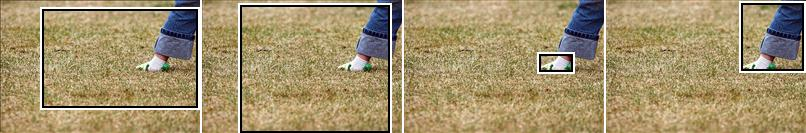
\includegraphics[width=1.9in,height=0.8in]{picture/badComparison/6_46_compare.jpg} \\
    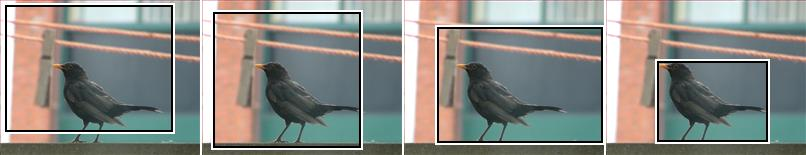
\includegraphics[width=1.9in,height=0.8in]{picture/badComparison/98_imCanvs_Compare.jpg}
    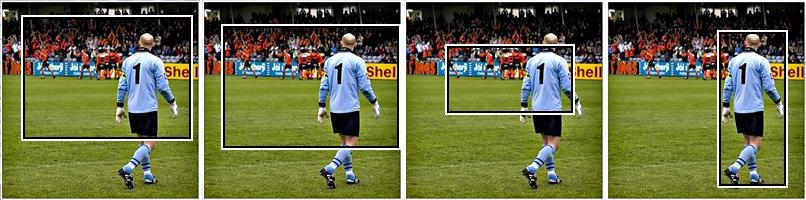
\includegraphics[width=1.9in,height=0.8in]{picture/badComparison/7_379_compare.jpg} \\
    \figcaption{\footnotesize (a) FG(Ma,2003) (b) SM(Itti,1998) (c) CRFM(Liu,2007) (d) Ground truth\vspace{0.3cm}  \\}
    \hrule
    \begin{thebibliography}{9}
        \tiny
        \bibitem{ConcreteMath} Liu, Tie, et al. "Learning to detect a salient object."\textit{ Computer Vision and Pattern Recognition, 2007. CVPR'07. IEEE Conference on. IEEE, 2007. }
    \end{thebibliography}
}

% End
\section{7 End}
\frame{
    \frametitle{Thank You! Suggestions and Questions Please.}
    \begin{center}
        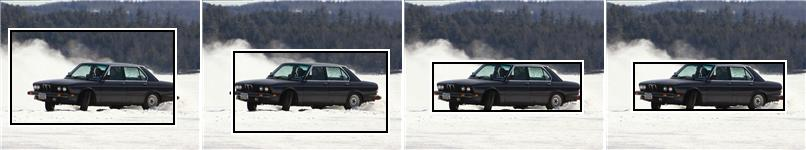
\includegraphics[width=2.8in,height=0.8in]{picture/perfectComparison/35_imCanvs_Compare.jpg} \\
        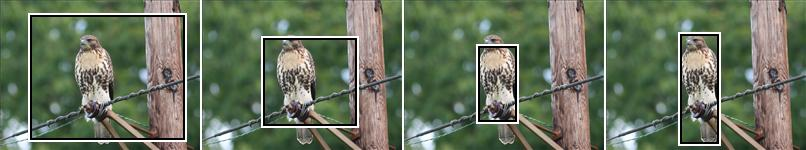
\includegraphics[width=2.8in,height=0.8in]{picture/sosoComparison/159_imCanvs_Compare.jpg} \\
        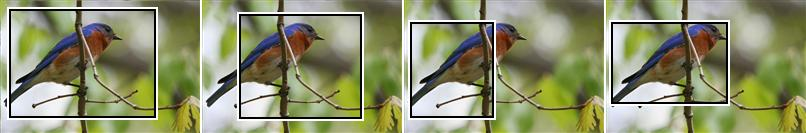
\includegraphics[width=2.8in,height=0.8in]{picture/badComparison/6_212_compare.jpg} \\
    \end{center}

            \hrule
    \begin{thebibliography}{9}
        \tiny
        \bibitem{ConcreteMath} Liu, Tie, et al. "Learning to detect a salient object."\textit{ Computer Vision and Pattern Recognition, 2007. CVPR'07. IEEE Conference on. IEEE, 2007. }
    \end{thebibliography}
}

\end{document}


